\anonsection{Заключение}

В рамках работы был создан прототип программы для FDTD-
моделирования, способный эффективно использовать ресурсы GPU. При
помощи разработанной программы была произведена тестовая симуляция рас-
пространения гармонического сигнала, излучаемого тонким симметричным
вибратором в замкнутом счётном объёме. Также была разработана референсная
ЦПУ-реализация и произведено сравнение производительности расчётов с ис-
пользованием ЦПУ и ГПУ.

В ходе работы было выяснено, что использование графических процессо-
ров обеспечивает увеличение производительности до 17 раз, причём в про-
граммном коде не был реализован выровненный доступ к памяти, что является
перспективным направлением разработки. Также, в отличие от CPU, произво-
дительность графических процессоров меньше зависит от размеров счётного
объёма.

\begin{figure}
    \centering
    \begin{subfigure}[b]{0.3\textwidth}
        
\includegraphics[width=\textwidth]{include/graphics/image6}

        \label{fig:gull}
    \end{subfigure}
    ~ %add desired spacing between images, e. g. ~, \quad, \qquad, \hfill etc. 
      %(or a blank line to force the subfigure onto a new line)
    \begin{subfigure}[b]{0.3\textwidth}
        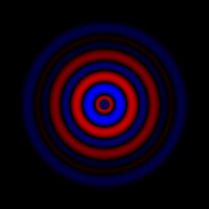
\includegraphics[width=\textwidth]{include/graphics/image7}
  
        \label{fig:tiger}
    \end{subfigure}
    ~ %add desired spacing between images, e. g. ~, \quad, \qquad, \hfill etc. 
    %(or a blank line to force the subfigure onto a new line)
    \begin{subfigure}[b]{0.3\textwidth}
        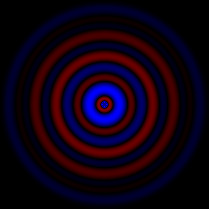
\includegraphics[width=\textwidth]{include/graphics/image8}

        \label{fig:mouse}
    \end{subfigure}
    
\bigskip
        \begin{subfigure}[b]{0.3\textwidth}
        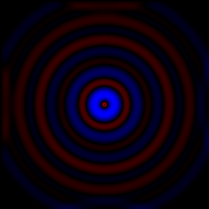
\includegraphics[width=\textwidth]{include/graphics/image9}

        \label{fig:gull}
    \end{subfigure}
    ~ %add desired spacing between images, e. g. ~, \quad, \qquad, \hfill etc. 
      %(or a blank line to force the subfigure onto a new line)
    \begin{subfigure}[b]{0.3\textwidth}
        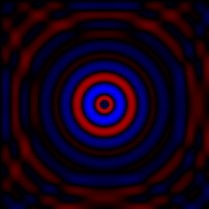
\includegraphics[width=\textwidth]{include/graphics/image10}
  
        \label{fig:tiger}
    \end{subfigure}
    ~ %add desired spacing between images, e. g. ~, \quad, \qquad, \hfill etc. 
    %(or a blank line to force the subfigure onto a new line)
    \begin{subfigure}[b]{0.3\textwidth}
        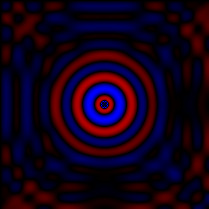
\includegraphics[width=\textwidth]{include/graphics/image11}

        \label{fig:mouse}
    \end{subfigure}

    \caption{Изменение электрического поля во времени (вид сверху)}\label{fig:animals}
\end{figure}
\clearpage
\begin{figure}[p]
\centering
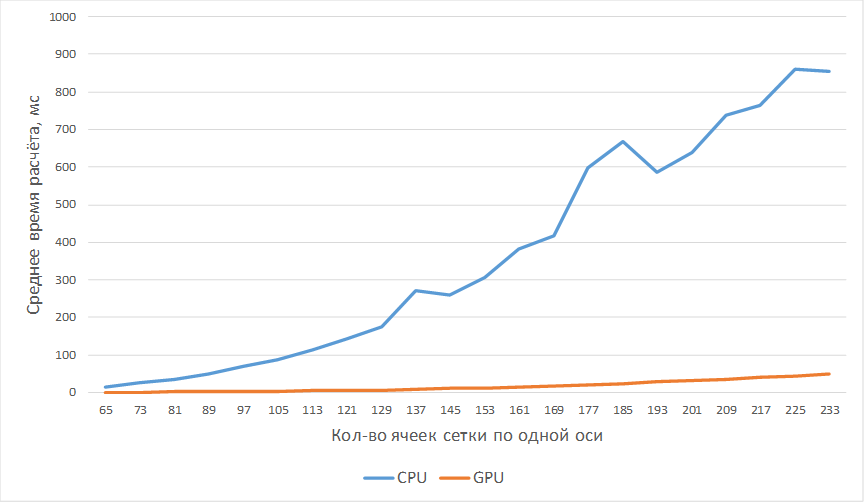
\includegraphics[width=0.95\textwidth]{include/graphics/image12}
\caption{Зависимость среднего времени расчёта компонент вектора магнитной напряжённости в конкретный момент времени во всех ячейках от размеров сетки}
\label{fig:1stComparsion}
\end{figure}
\begin{figure}[p]
\centering
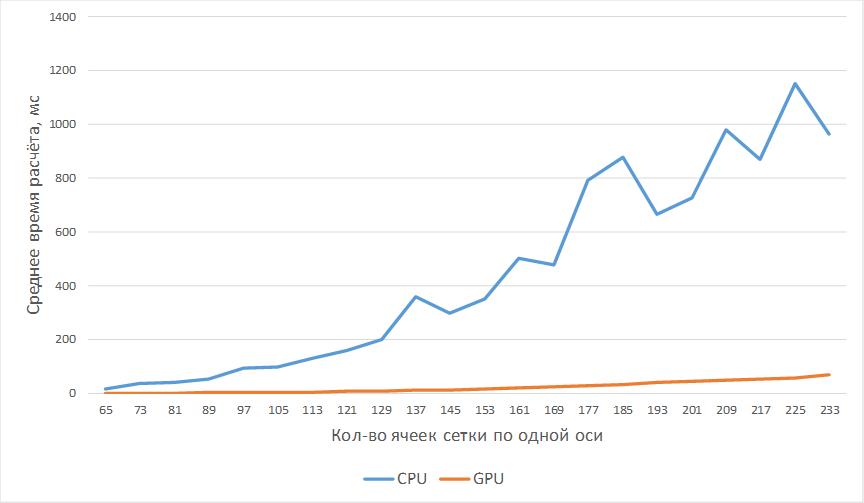
\includegraphics[width=0.95\textwidth]{include/graphics/image13}
\caption{Зависимость среднего времени расчёта компонент вектора электрической напряжённости в конкретный момент времени во всех ячейках от размеров сетки}
\label{fig:2ndComparsion}
\end{figure}

\clearpage